\index{wing nuts}
\index{filament spool}
\index{spool}
\glossary{Spool}{Plastic Filament coiled and stored on a plastic reel. Preferred due to improved feeding and better mounting options.}
\glossary{Filament}{Plastic material in "string" like form, as is fed to the printer.}
\glossary{ABS}{Acrylonitrile Butadiene Styrene thermoplastic. Usually extrudes at 230C.}
\glossary{PLA}{Polylactic Acid is a corn-based biodegradable polymer. Usually extrudes at 185C.}
\glossary{HDPE}{High Density Polyethylene.}
\glossary{Polycarbonate}{A strong and impact resistant thermoplastic. Usually extrudes at ~300C.}
\glossary{HIPS}{High Impact Polystyrene.}
\glossary{Laywoo-D3}{Wooden filament similar to PLA. Contains 40 percent recycled wood. Usually prints at ~180C- 210C. Color can be changed by varying the extrusion temperature.}

Before you start printing you will need to load a reel of filamant on to the reel holder. If mounted correctly the reel holder will keep the filament reel rotating smoothly. The reel holder is meant to work with 1kg and 5lb plastic filament reels but can be modified the work with other reel and spool types.

\begin{enumerate}

\item Locate the filament reel spindle and unthread and remove the wingnut and washer (fig. \ref{fig:spool_mount_parts}, page \pageref{fig:spool_mount_parts}). Set the filament reel with the filament feeding counter clockwise. Insert the reel spindle into the plastic filament reel.

\begin{figure}[H]
\centering
\includegraphics[keepaspectratio=true,angle=0,height=0.4\textheight,width=1.0\textwidth]{spool_mount_parts.JPG}
\caption{Filament spool mount parts}
\label{fig:spool_mount_parts}
\end{figure}

\item Thread the reel spindle into the filament holder mounted on the lower right hand side of the TAZ 3D Printer (fig. \ref{fig:filament_spool_mount_front}, page \pageref{fig:filament_spool_mount_front}). Turn the spindle handle clockwise until it snugs up against the reel and then turn it back one quarter of a turn. This will allow the reel to easily turn but not turn too freely that it would allow the filament to unravel.

\begin{figure}[hp]
\centering
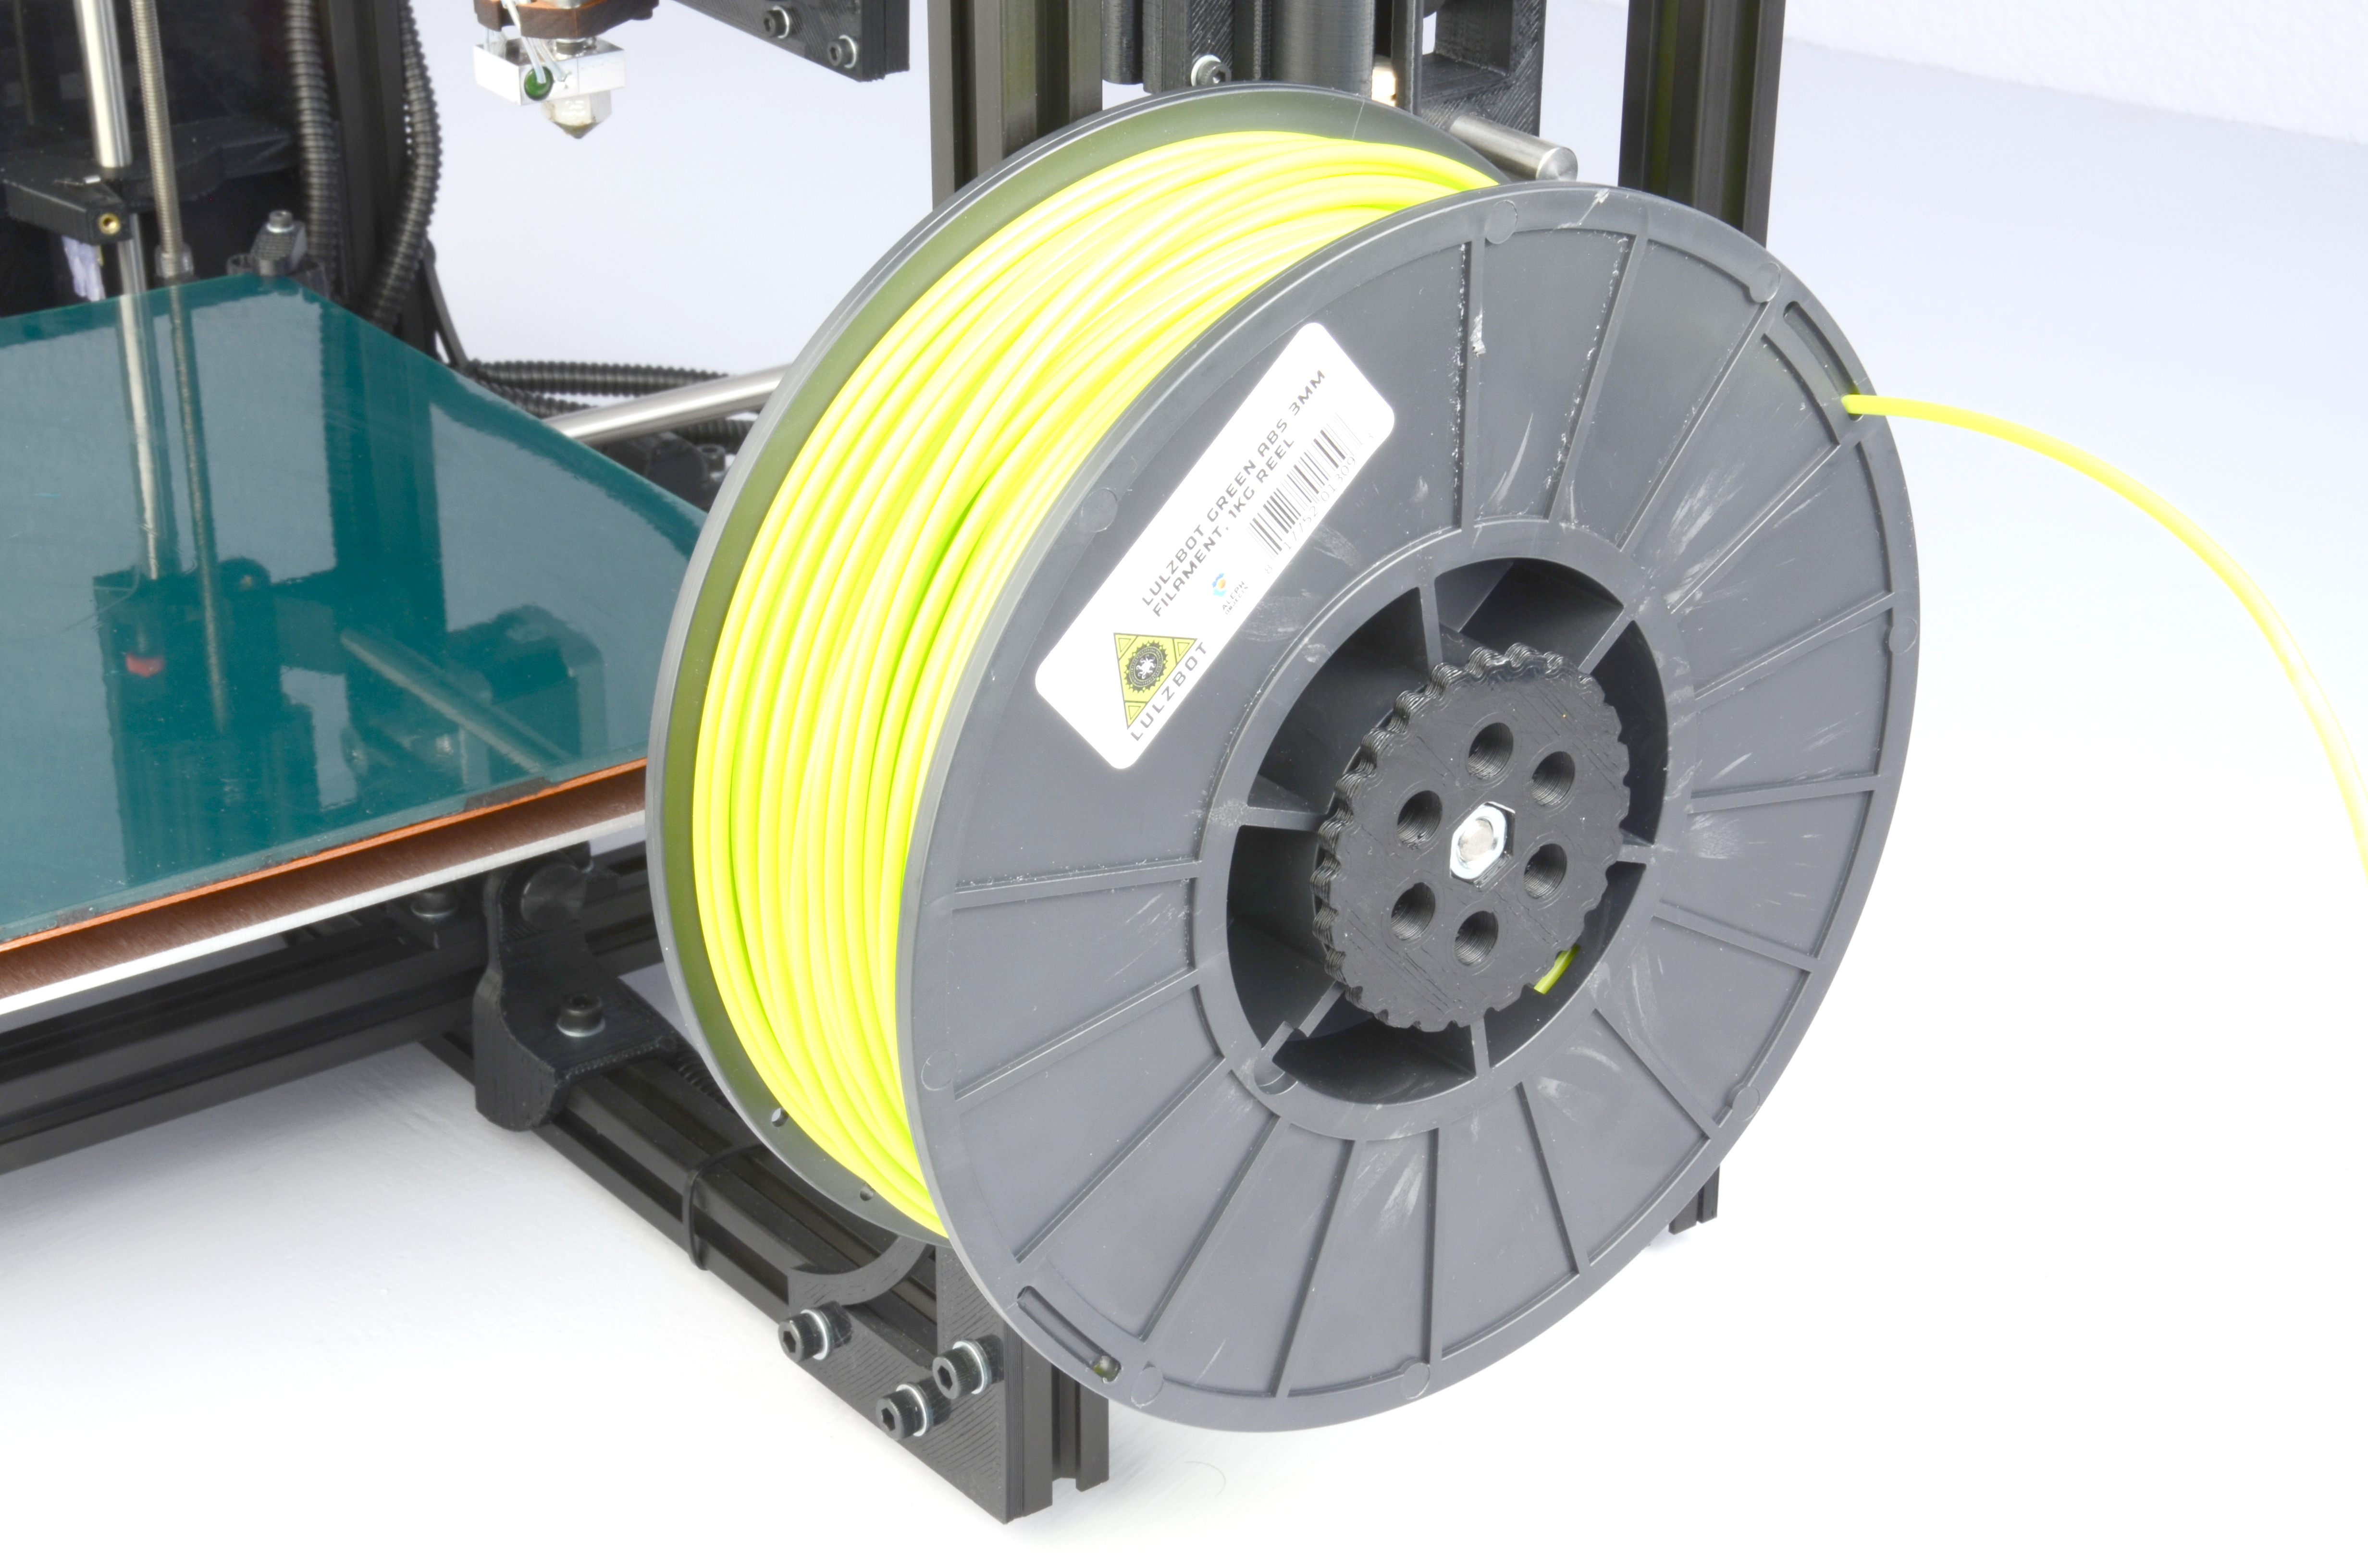
\includegraphics[keepaspectratio=true,angle=0,height=0.4\textheight,width=1.0\textwidth]{filament_spool_mount_front.JPG}
\caption{Filament spool mount front}
\label{fig:filament_spool_mount_front}
\end{figure}

\begin{figure}[hp]
\centering
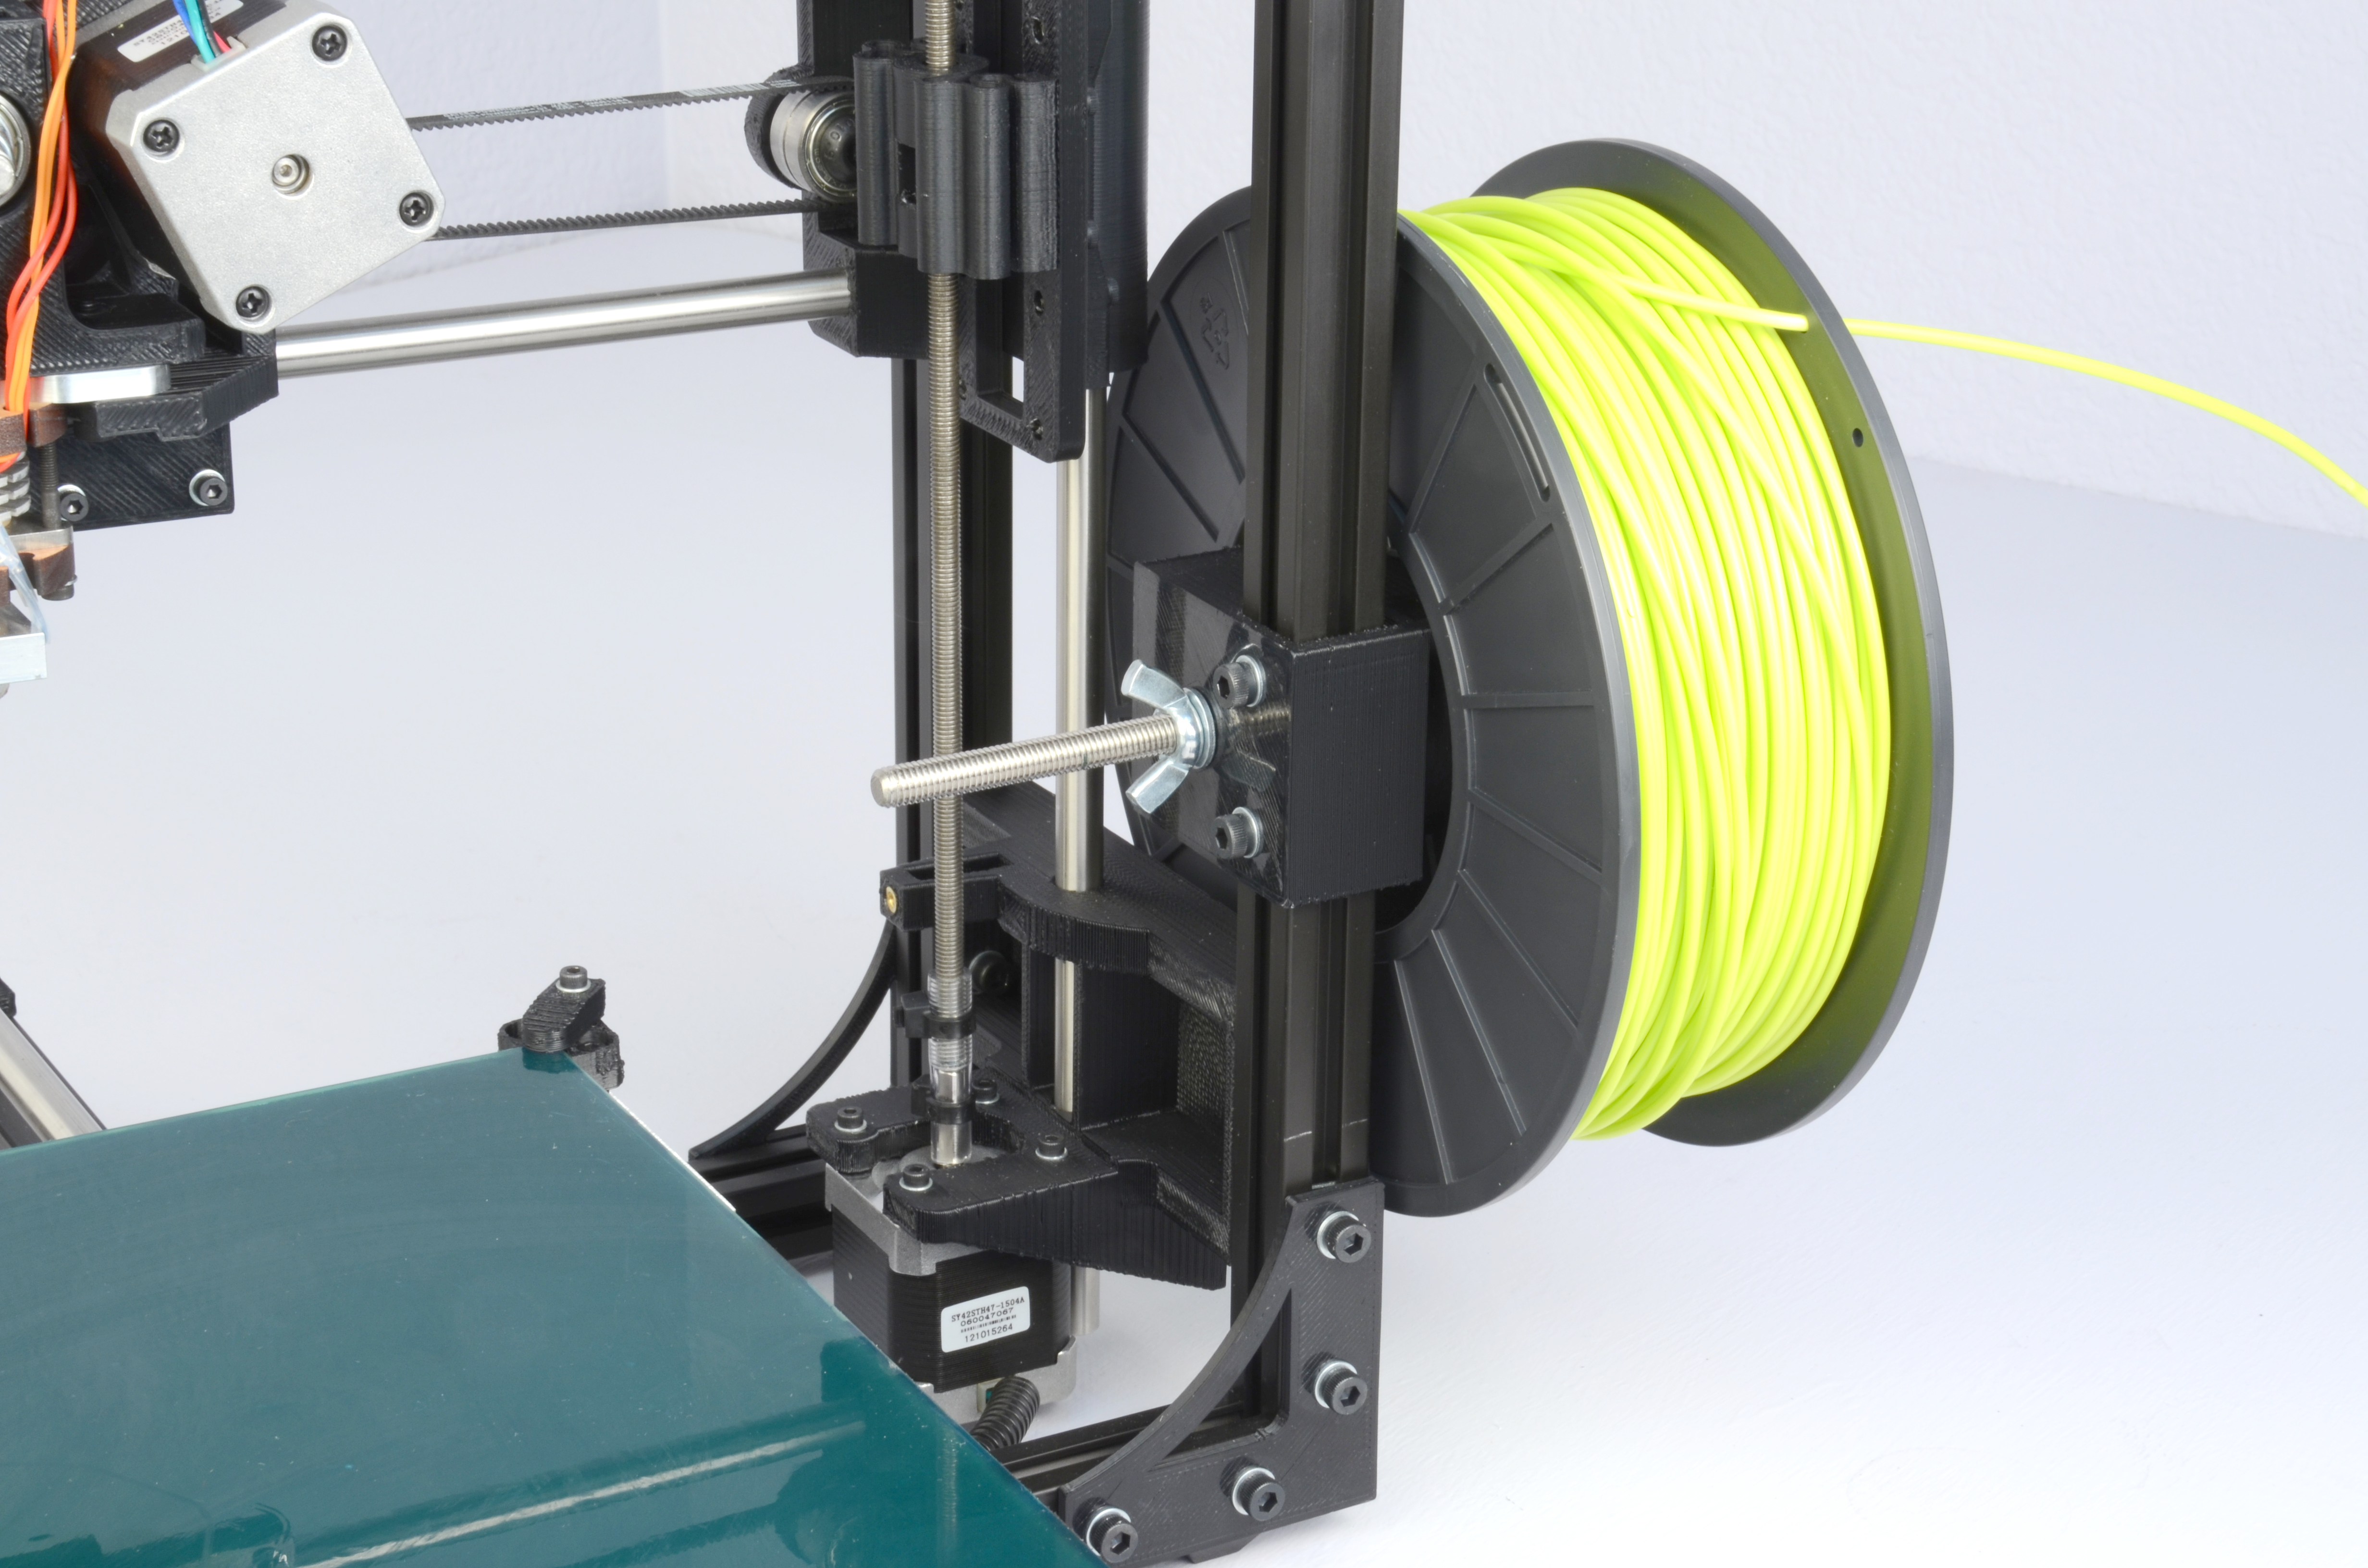
\includegraphics[keepaspectratio=true,angle=0,height=0.4\textheight,width=1.0\textwidth]{filament_spool_mount_back.JPG}
\caption{Filament spool mount back}
\label{fig:filament_spool_mount_back}
\end{figure}

\item Slide the washer onto the end of the spindle on the back of the reel mount. Thread the wing nut onto the spindle end and loosely up against the nut on the back of the reel mount (fig. \ref{fig:filament_spool_mount_back}, page \pageref{fig:filament_spool_mount_back}). While holding the reel spindle handle in place tighten the wing nut against the nut on the back of the reel mount. This will keep the tension you set at the handle in place. If you need to adjust the tension, loosen the wingnut, adjust the handle tension, and retighten the wingnut.

\index{feed tube}
\item Feed the end of the filament through the filament feed tube. The Filament should now be threaded through the PTFE sleeve and exiting near the extruder (fig. \ref{fig:filament_in_guide}, page \pageref{fig:filament_in_guide}).

\begin{figure}[H]
\centering
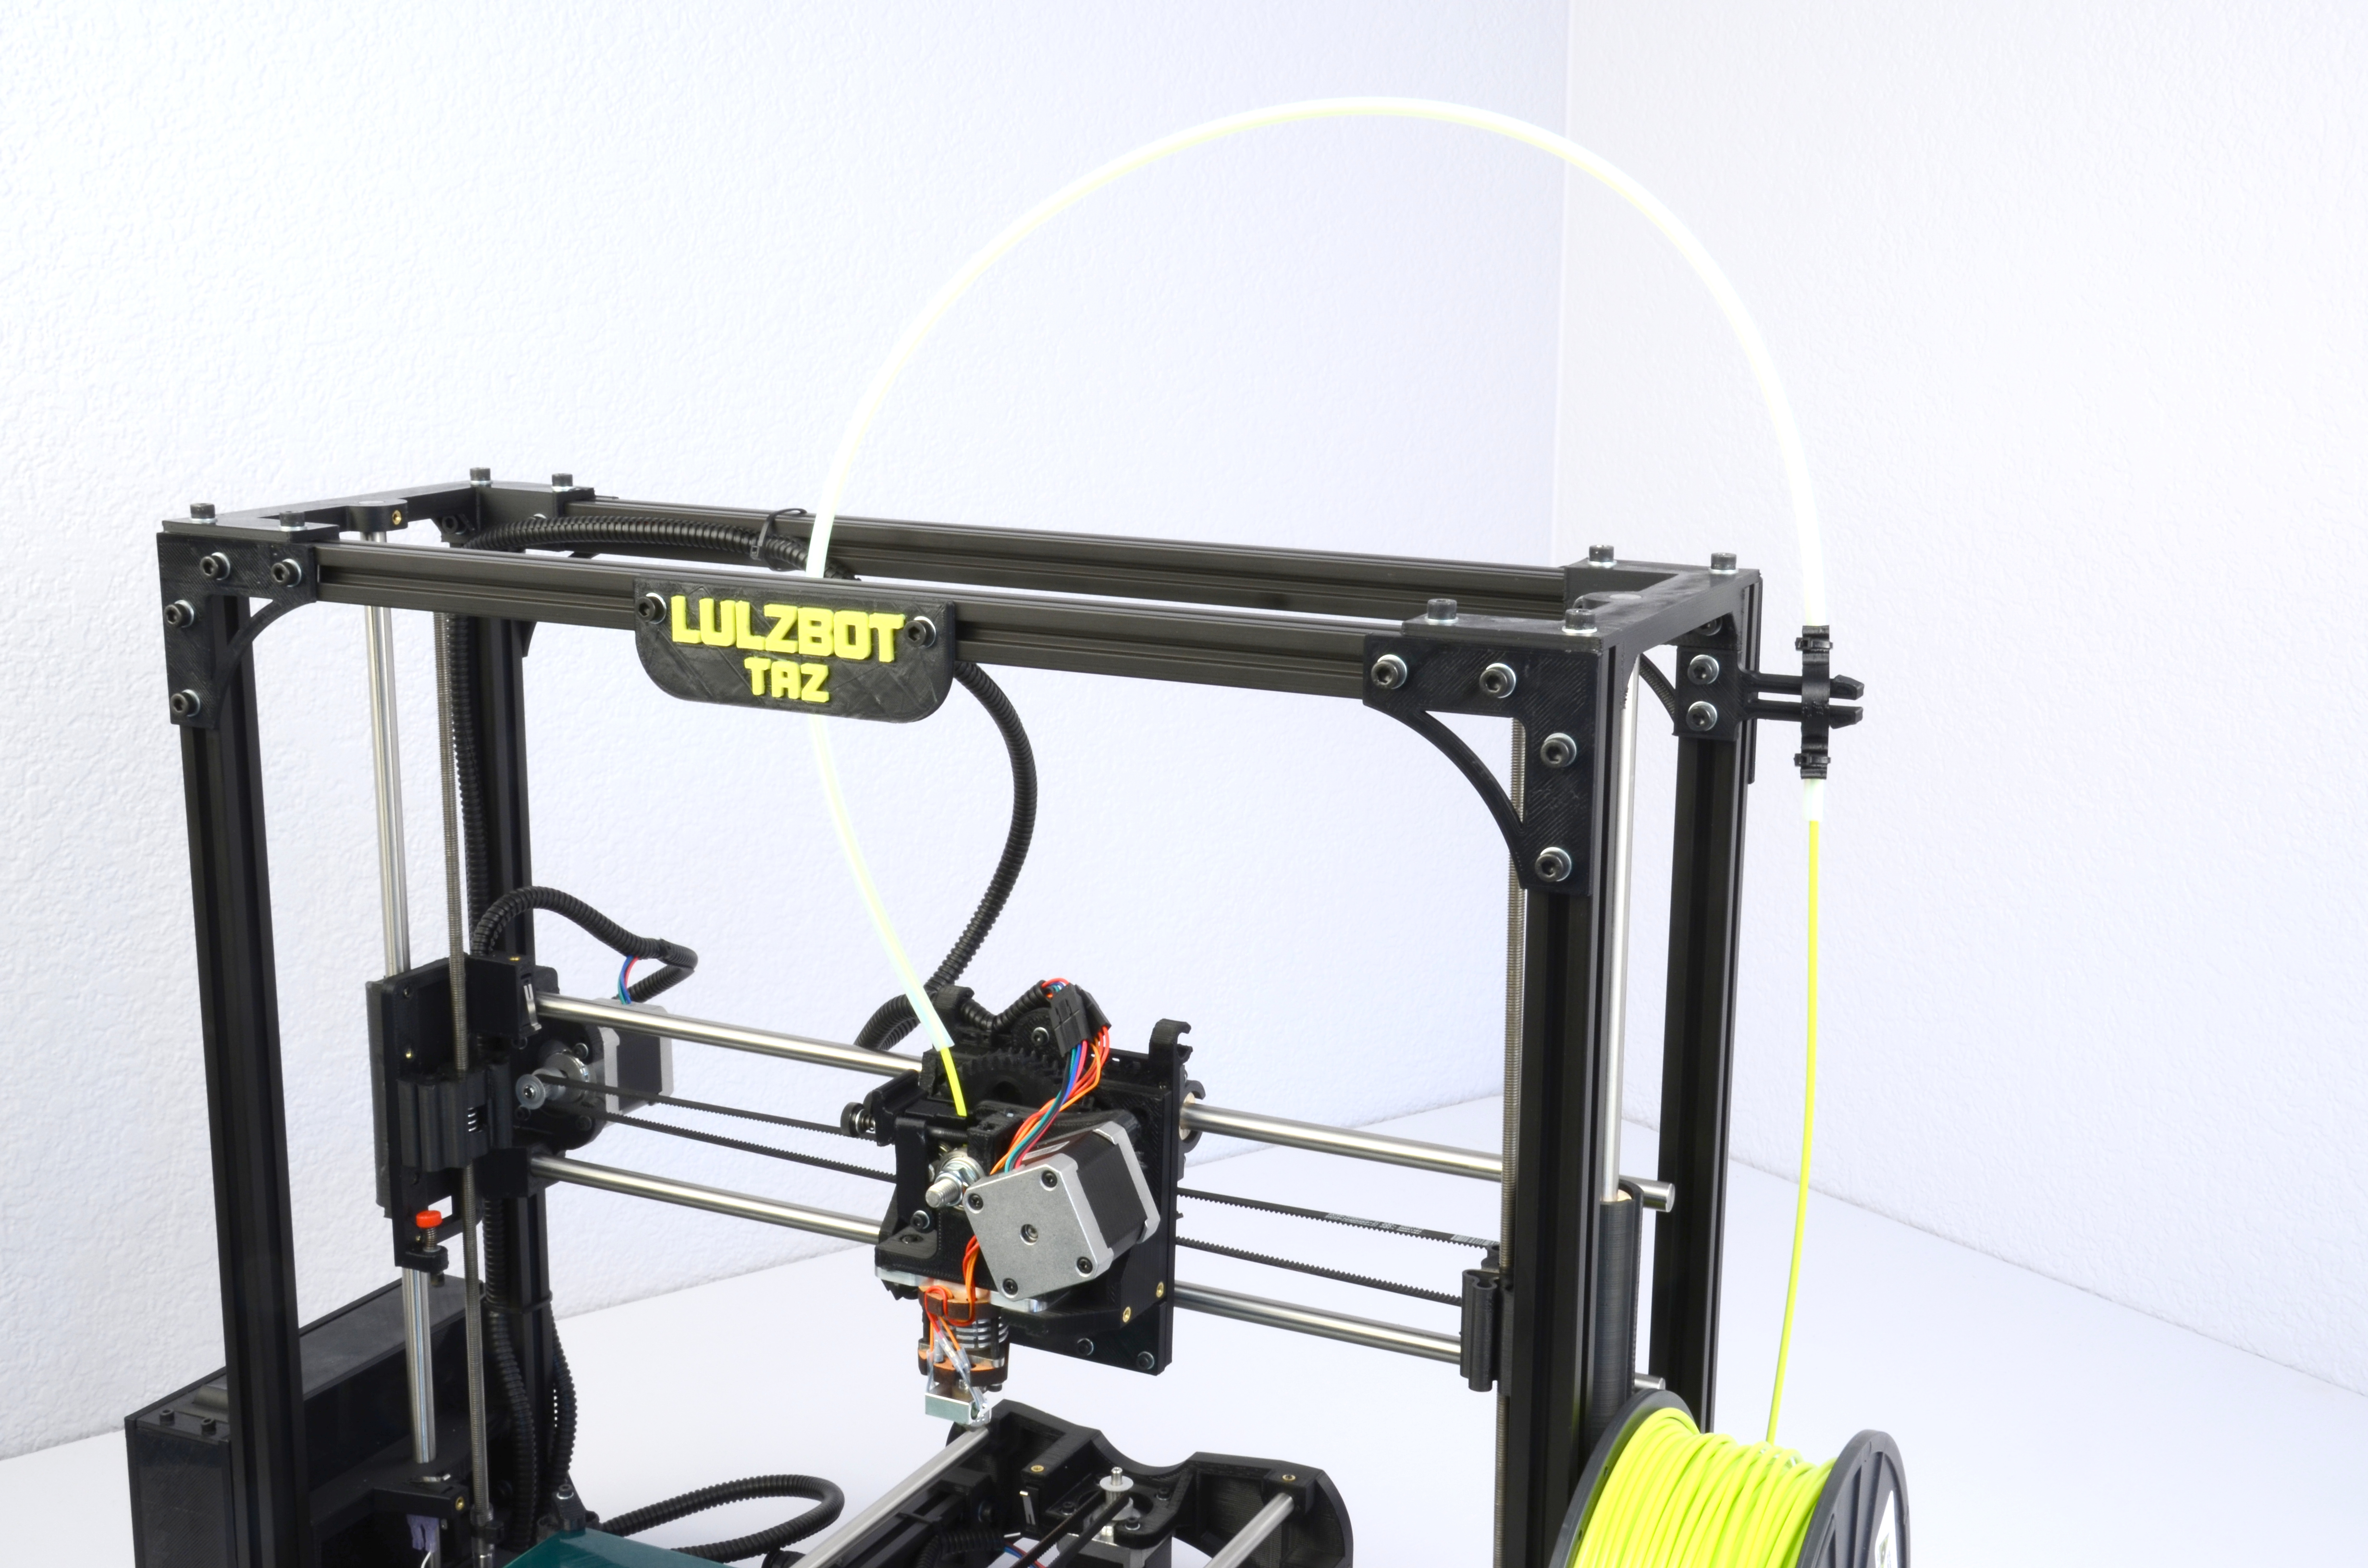
\includegraphics[keepaspectratio=true,angle=0,height=0.4\textheight,width=1.0\textwidth]{filament_in_guide.JPG}
\caption{Filament run through the guide}
\label{fig:filament_in_guide}
\end{figure}

\item When changing filament, slide the opposite end of the filament through one of the holes in hub of the filament spool. This will keep the filament from unwinding from the spool (fig. \ref{fig:filament_spool_mount_front}, page \pageref{fig:filament_spool_mount_front}).

\end{enumerate}
